% Options for packages loaded elsewhere
\PassOptionsToPackage{unicode}{hyperref}
\PassOptionsToPackage{hyphens}{url}
%
\documentclass[
]{article}
\usepackage{lmodern}
\usepackage{amssymb,amsmath}
\usepackage{ifxetex,ifluatex}
\ifnum 0\ifxetex 1\fi\ifluatex 1\fi=0 % if pdftex
  \usepackage[T1]{fontenc}
  \usepackage[utf8]{inputenc}
  \usepackage{textcomp} % provide euro and other symbols
\else % if luatex or xetex
  \usepackage{unicode-math}
  \defaultfontfeatures{Scale=MatchLowercase}
  \defaultfontfeatures[\rmfamily]{Ligatures=TeX,Scale=1}
\fi
% Use upquote if available, for straight quotes in verbatim environments
\IfFileExists{upquote.sty}{\usepackage{upquote}}{}
\IfFileExists{microtype.sty}{% use microtype if available
  \usepackage[]{microtype}
  \UseMicrotypeSet[protrusion]{basicmath} % disable protrusion for tt fonts
}{}
\makeatletter
\@ifundefined{KOMAClassName}{% if non-KOMA class
  \IfFileExists{parskip.sty}{%
    \usepackage{parskip}
  }{% else
    \setlength{\parindent}{0pt}
    \setlength{\parskip}{6pt plus 2pt minus 1pt}}
}{% if KOMA class
  \KOMAoptions{parskip=half}}
\makeatother
\usepackage{xcolor}
\IfFileExists{xurl.sty}{\usepackage{xurl}}{} % add URL line breaks if available
\IfFileExists{bookmark.sty}{\usepackage{bookmark}}{\usepackage{hyperref}}
\hypersetup{
  pdftitle={TP2},
  pdfauthor={Alison Hourdeau},
  hidelinks,
  pdfcreator={LaTeX via pandoc}}
\urlstyle{same} % disable monospaced font for URLs
\usepackage[margin=1in]{geometry}
\usepackage{color}
\usepackage{fancyvrb}
\newcommand{\VerbBar}{|}
\newcommand{\VERB}{\Verb[commandchars=\\\{\}]}
\DefineVerbatimEnvironment{Highlighting}{Verbatim}{commandchars=\\\{\}}
% Add ',fontsize=\small' for more characters per line
\usepackage{framed}
\definecolor{shadecolor}{RGB}{248,248,248}
\newenvironment{Shaded}{\begin{snugshade}}{\end{snugshade}}
\newcommand{\AlertTok}[1]{\textcolor[rgb]{0.94,0.16,0.16}{#1}}
\newcommand{\AnnotationTok}[1]{\textcolor[rgb]{0.56,0.35,0.01}{\textbf{\textit{#1}}}}
\newcommand{\AttributeTok}[1]{\textcolor[rgb]{0.77,0.63,0.00}{#1}}
\newcommand{\BaseNTok}[1]{\textcolor[rgb]{0.00,0.00,0.81}{#1}}
\newcommand{\BuiltInTok}[1]{#1}
\newcommand{\CharTok}[1]{\textcolor[rgb]{0.31,0.60,0.02}{#1}}
\newcommand{\CommentTok}[1]{\textcolor[rgb]{0.56,0.35,0.01}{\textit{#1}}}
\newcommand{\CommentVarTok}[1]{\textcolor[rgb]{0.56,0.35,0.01}{\textbf{\textit{#1}}}}
\newcommand{\ConstantTok}[1]{\textcolor[rgb]{0.00,0.00,0.00}{#1}}
\newcommand{\ControlFlowTok}[1]{\textcolor[rgb]{0.13,0.29,0.53}{\textbf{#1}}}
\newcommand{\DataTypeTok}[1]{\textcolor[rgb]{0.13,0.29,0.53}{#1}}
\newcommand{\DecValTok}[1]{\textcolor[rgb]{0.00,0.00,0.81}{#1}}
\newcommand{\DocumentationTok}[1]{\textcolor[rgb]{0.56,0.35,0.01}{\textbf{\textit{#1}}}}
\newcommand{\ErrorTok}[1]{\textcolor[rgb]{0.64,0.00,0.00}{\textbf{#1}}}
\newcommand{\ExtensionTok}[1]{#1}
\newcommand{\FloatTok}[1]{\textcolor[rgb]{0.00,0.00,0.81}{#1}}
\newcommand{\FunctionTok}[1]{\textcolor[rgb]{0.00,0.00,0.00}{#1}}
\newcommand{\ImportTok}[1]{#1}
\newcommand{\InformationTok}[1]{\textcolor[rgb]{0.56,0.35,0.01}{\textbf{\textit{#1}}}}
\newcommand{\KeywordTok}[1]{\textcolor[rgb]{0.13,0.29,0.53}{\textbf{#1}}}
\newcommand{\NormalTok}[1]{#1}
\newcommand{\OperatorTok}[1]{\textcolor[rgb]{0.81,0.36,0.00}{\textbf{#1}}}
\newcommand{\OtherTok}[1]{\textcolor[rgb]{0.56,0.35,0.01}{#1}}
\newcommand{\PreprocessorTok}[1]{\textcolor[rgb]{0.56,0.35,0.01}{\textit{#1}}}
\newcommand{\RegionMarkerTok}[1]{#1}
\newcommand{\SpecialCharTok}[1]{\textcolor[rgb]{0.00,0.00,0.00}{#1}}
\newcommand{\SpecialStringTok}[1]{\textcolor[rgb]{0.31,0.60,0.02}{#1}}
\newcommand{\StringTok}[1]{\textcolor[rgb]{0.31,0.60,0.02}{#1}}
\newcommand{\VariableTok}[1]{\textcolor[rgb]{0.00,0.00,0.00}{#1}}
\newcommand{\VerbatimStringTok}[1]{\textcolor[rgb]{0.31,0.60,0.02}{#1}}
\newcommand{\WarningTok}[1]{\textcolor[rgb]{0.56,0.35,0.01}{\textbf{\textit{#1}}}}
\usepackage{graphicx,grffile}
\makeatletter
\def\maxwidth{\ifdim\Gin@nat@width>\linewidth\linewidth\else\Gin@nat@width\fi}
\def\maxheight{\ifdim\Gin@nat@height>\textheight\textheight\else\Gin@nat@height\fi}
\makeatother
% Scale images if necessary, so that they will not overflow the page
% margins by default, and it is still possible to overwrite the defaults
% using explicit options in \includegraphics[width, height, ...]{}
\setkeys{Gin}{width=\maxwidth,height=\maxheight,keepaspectratio}
% Set default figure placement to htbp
\makeatletter
\def\fps@figure{htbp}
\makeatother
\setlength{\emergencystretch}{3em} % prevent overfull lines
\providecommand{\tightlist}{%
  \setlength{\itemsep}{0pt}\setlength{\parskip}{0pt}}
\setcounter{secnumdepth}{-\maxdimen} % remove section numbering

\title{TP2}
\author{Alison Hourdeau}
\date{17/03/2021}

\begin{document}
\maketitle

\#1. Evaluation de la règle de classement (iris de Fisher) \#\#1.
Diagnostic apparent

On charge le TP1 pour avoir tous les résultats précédents.

\begin{Shaded}
\begin{Highlighting}[]
\KeywordTok{library}\NormalTok{(}\StringTok{"knitr"}\NormalTok{)}
\KeywordTok{purl}\NormalTok{(}\StringTok{"corrige_TP1.Rmd"}\NormalTok{)}
\end{Highlighting}
\end{Shaded}

\begin{verbatim}
## [1] "corrige_TP1.R"
\end{verbatim}

\begin{Shaded}
\begin{Highlighting}[]
\KeywordTok{source}\NormalTok{(}\StringTok{"corrige_TP1.R"}\NormalTok{)}
\end{Highlighting}
\end{Shaded}

\begin{verbatim}
## List of 9
##  $ statistic: Named num 5.36
##   ..- attr(*, "names")= chr "X-squared"
##  $ parameter: Named int 3
##   ..- attr(*, "names")= chr "df"
##  $ p.value  : num 0.147
##  $ method   : chr "Pearson's Chi-squared test"
##  $ data.name: chr "V3V1"
##  $ observed : num [1:4, 1:2] 30 30 10 10 20 20 15 15
##  $ expected : num [1:4, 1:2] 26.7 26.7 13.3 13.3 23.3 ...
##  $ residuals: num [1:4, 1:2] 0.645 0.645 -0.913 -0.913 -0.69 ...
##  $ stdres   : num [1:4, 1:2] 1.16 1.16 -1.46 -1.46 -1.16 ...
##  - attr(*, "class")= chr "htest"
\end{verbatim}

\begin{verbatim}
## 
## Attaching package: 'dplyr'
\end{verbatim}

\begin{verbatim}
## The following objects are masked from 'package:stats':
## 
##     filter, lag
\end{verbatim}

\begin{verbatim}
## The following objects are masked from 'package:base':
## 
##     intersect, setdiff, setequal, union
\end{verbatim}

\begin{verbatim}
## Registered S3 method overwritten by 'GGally':
##   method from   
##   +.gg   ggplot2
\end{verbatim}

\begin{verbatim}
## ------------------------------------------------
##  MBox Chi-sqr. df P
## ------------------------------------------------
##   146.6632   140.9430          20       0.0000
## ------------------------------------------------
## Covariance matrices are significantly different.
\end{verbatim}

\includegraphics{TP2_files/figure-latex/unnamed-chunk-1-1.pdf}
\includegraphics{TP2_files/figure-latex/unnamed-chunk-1-2.pdf}

On calcule la matrice de confusion à l'aide de la fonction table sur la
classe réelle et la classe prédite.

\begin{Shaded}
\begin{Highlighting}[]
\KeywordTok{table}\NormalTok{(}\DataTypeTok{Yreel =}\NormalTok{ iris}\OperatorTok{$}\NormalTok{Y,}\DataTypeTok{Ypredit =}\NormalTok{ Ypredit)}
\end{Highlighting}
\end{Shaded}

\begin{verbatim}
##             Ypredit
## Yreel        setosa versicolor virginica
##   setosa         50          0         0
##   versicolor      0         48         2
##   virginica       0          1        49
\end{verbatim}

On calcule le taux de bon classement (TBC) :

\begin{Shaded}
\begin{Highlighting}[]
\NormalTok{TBC=}\KeywordTok{mean}\NormalTok{(iris}\OperatorTok{$}\NormalTok{Y}\OperatorTok{==}\NormalTok{Ypredit)}
\NormalTok{TBC}
\end{Highlighting}
\end{Shaded}

\begin{verbatim}
## [1] 0.98
\end{verbatim}

Puis le taux de mauvais classement (TMC) :

\begin{Shaded}
\begin{Highlighting}[]
\NormalTok{TMC =}\StringTok{ }\DecValTok{1} \OperatorTok{-}\StringTok{ }\NormalTok{TBC}
\NormalTok{TMC}
\end{Highlighting}
\end{Shaded}

\begin{verbatim}
## [1] 0.02
\end{verbatim}

La méthode utilisée peut souffrir d'un biais d'optimisme car les données
ont servi à apprendre le modèle et à le tester. Pour avoir ne pas avoir
de biais, on peut découper les données en deux échantillons : un
échantillon d'apprentissage (environ 2/3 à 75\% de l'échantillon global)
et un échantillon test.

\#\#2. Diagnostic sur un échantillon test

On découpe les données iris en un échantillon d'apprentissage (70\% des
données) et un échantillon test (30\% des données) pour construire le
tableau de score :

\begin{Shaded}
\begin{Highlighting}[]
\NormalTok{n =}\StringTok{ }\KeywordTok{nrow}\NormalTok{(iris)}
\KeywordTok{set.seed}\NormalTok{(}\DecValTok{1234}\NormalTok{)}

\CommentTok{#Tirage}
\NormalTok{idx=}\KeywordTok{sample}\NormalTok{(n,}\KeywordTok{round}\NormalTok{(n}\OperatorTok{*}\FloatTok{0.7}\NormalTok{),}\DataTypeTok{replace=}\OtherTok{FALSE}\NormalTok{)}

\CommentTok{#Echantillon d'apprentissage}
\NormalTok{iristrain=iris[idx,]}
\NormalTok{iristrain}
\end{Highlighting}
\end{Shaded}

\begin{verbatim}
##      X1  X2  X3  X4          Y
## 28  5.2 3.5 1.5 0.2     setosa
## 80  5.7 2.6 3.5 1.0 versicolor
## 101 6.3 3.3 6.0 2.5  virginica
## 111 6.5 3.2 5.1 2.0  virginica
## 137 6.3 3.4 5.6 2.4  virginica
## 133 6.4 2.8 5.6 2.2  virginica
## 144 6.8 3.2 5.9 2.3  virginica
## 132 7.9 3.8 6.4 2.0  virginica
## 98  6.2 2.9 4.3 1.3 versicolor
## 103 7.1 3.0 5.9 2.1  virginica
## 90  5.5 2.5 4.0 1.3 versicolor
## 70  5.6 2.5 3.9 1.1 versicolor
## 79  6.0 2.9 4.5 1.5 versicolor
## 116 6.4 3.2 5.3 2.3  virginica
## 14  4.3 3.0 1.1 0.1     setosa
## 126 7.2 3.2 6.0 1.8  virginica
## 62  5.9 3.0 4.2 1.5 versicolor
## 4   4.6 3.1 1.5 0.2     setosa
## 143 5.8 2.7 5.1 1.9  virginica
## 40  5.1 3.4 1.5 0.2     setosa
## 93  5.8 2.6 4.0 1.2 versicolor
## 122 5.6 2.8 4.9 2.0  virginica
## 5   5.0 3.6 1.4 0.2     setosa
## 66  6.7 3.1 4.4 1.4 versicolor
## 135 6.1 2.6 5.6 1.4  virginica
## 47  5.1 3.8 1.6 0.2     setosa
## 131 7.4 2.8 6.1 1.9  virginica
## 123 7.7 2.8 6.7 2.0  virginica
## 84  6.0 2.7 5.1 1.6 versicolor
## 48  4.6 3.2 1.4 0.2     setosa
## 108 7.3 2.9 6.3 1.8  virginica
## 3   4.7 3.2 1.3 0.2     setosa
## 87  6.7 3.1 4.7 1.5 versicolor
## 41  5.0 3.5 1.3 0.3     setosa
## 115 5.8 2.8 5.1 2.4  virginica
## 100 5.7 2.8 4.1 1.3 versicolor
## 72  6.1 2.8 4.0 1.3 versicolor
## 32  5.4 3.4 1.5 0.4     setosa
## 42  4.5 2.3 1.3 0.3     setosa
## 43  4.4 3.2 1.3 0.2     setosa
## 2   4.9 3.0 1.4 0.2     setosa
## 138 6.4 3.1 5.5 1.8  virginica
## 54  5.5 2.3 4.0 1.3 versicolor
## 49  5.3 3.7 1.5 0.2     setosa
## 102 5.8 2.7 5.1 1.9  virginica
## 56  5.7 2.8 4.5 1.3 versicolor
## 51  7.0 3.2 4.7 1.4 versicolor
## 6   5.4 3.9 1.7 0.4     setosa
## 107 4.9 2.5 4.5 1.7  virginica
## 130 7.2 3.0 5.8 1.6  virginica
## 96  5.7 3.0 4.2 1.2 versicolor
## 106 7.6 3.0 6.6 2.1  virginica
## 57  6.3 3.3 4.7 1.6 versicolor
## 8   5.0 3.4 1.5 0.2     setosa
## 26  5.0 3.0 1.6 0.2     setosa
## 17  5.4 3.9 1.3 0.4     setosa
## 63  6.0 2.2 4.0 1.0 versicolor
## 97  5.7 2.9 4.2 1.3 versicolor
## 22  5.1 3.7 1.5 0.4     setosa
## 35  4.9 3.1 1.5 0.2     setosa
## 117 6.5 3.0 5.5 1.8  virginica
## 149 6.2 3.4 5.4 2.3  virginica
## 119 7.7 2.6 6.9 2.3  virginica
## 86  6.0 3.4 4.5 1.6 versicolor
## 142 6.9 3.1 5.1 2.3  virginica
## 10  4.9 3.1 1.5 0.1     setosa
## 55  6.5 2.8 4.6 1.5 versicolor
## 92  6.1 3.0 4.6 1.4 versicolor
## 25  4.8 3.4 1.9 0.2     setosa
## 88  6.3 2.3 4.4 1.3 versicolor
## 50  5.0 3.3 1.4 0.2     setosa
## 139 6.0 3.0 4.8 1.8  virginica
## 20  5.1 3.8 1.5 0.3     setosa
## 140 6.9 3.1 5.4 2.1  virginica
## 94  5.0 2.3 3.3 1.0 versicolor
## 71  5.9 3.2 4.8 1.8 versicolor
## 61  5.0 2.0 3.5 1.0 versicolor
## 104 6.3 2.9 5.6 1.8  virginica
## 109 6.7 2.5 5.8 1.8  virginica
## 27  5.0 3.4 1.6 0.4     setosa
## 121 6.9 3.2 5.7 2.3  virginica
## 60  5.2 2.7 3.9 1.4 versicolor
## 65  5.6 2.9 3.6 1.3 versicolor
## 36  5.0 3.2 1.2 0.2     setosa
## 150 5.9 3.0 5.1 1.8  virginica
## 19  5.7 3.8 1.7 0.3     setosa
## 9   4.4 2.9 1.4 0.2     setosa
## 134 6.3 2.8 5.1 1.5  virginica
## 30  4.7 3.2 1.6 0.2     setosa
## 52  6.4 3.2 4.5 1.5 versicolor
## 95  5.6 2.7 4.2 1.3 versicolor
## 38  4.9 3.6 1.4 0.1     setosa
## 83  5.8 2.7 3.9 1.2 versicolor
## 141 6.7 3.1 5.6 2.4  virginica
## 21  5.4 3.4 1.7 0.2     setosa
## 105 6.5 3.0 5.8 2.2  virginica
## 113 6.8 3.0 5.5 2.1  virginica
## 13  4.8 3.0 1.4 0.1     setosa
## 69  6.2 2.2 4.5 1.5 versicolor
## 110 7.2 3.6 6.1 2.5  virginica
## 118 7.7 3.8 6.7 2.2  virginica
## 73  6.3 2.5 4.9 1.5 versicolor
## 16  5.7 4.4 1.5 0.4     setosa
## 11  5.4 3.7 1.5 0.2     setosa
## 67  5.6 3.0 4.5 1.5 versicolor
\end{verbatim}

\begin{Shaded}
\begin{Highlighting}[]
\CommentTok{#Echantillon test}
\NormalTok{iristest=iris[}\OperatorTok{-}\NormalTok{idx,]}
\NormalTok{iristest}
\end{Highlighting}
\end{Shaded}

\begin{verbatim}
##      X1  X2  X3  X4          Y
## 1   5.1 3.5 1.4 0.2     setosa
## 7   4.6 3.4 1.4 0.3     setosa
## 12  4.8 3.4 1.6 0.2     setosa
## 15  5.8 4.0 1.2 0.2     setosa
## 18  5.1 3.5 1.4 0.3     setosa
## 23  4.6 3.6 1.0 0.2     setosa
## 24  5.1 3.3 1.7 0.5     setosa
## 29  5.2 3.4 1.4 0.2     setosa
## 31  4.8 3.1 1.6 0.2     setosa
## 33  5.2 4.1 1.5 0.1     setosa
## 34  5.5 4.2 1.4 0.2     setosa
## 37  5.5 3.5 1.3 0.2     setosa
## 39  4.4 3.0 1.3 0.2     setosa
## 44  5.0 3.5 1.6 0.6     setosa
## 45  5.1 3.8 1.9 0.4     setosa
## 46  4.8 3.0 1.4 0.3     setosa
## 53  6.9 3.1 4.9 1.5 versicolor
## 58  4.9 2.4 3.3 1.0 versicolor
## 59  6.6 2.9 4.6 1.3 versicolor
## 64  6.1 2.9 4.7 1.4 versicolor
## 68  5.8 2.7 4.1 1.0 versicolor
## 74  6.1 2.8 4.7 1.2 versicolor
## 75  6.4 2.9 4.3 1.3 versicolor
## 76  6.6 3.0 4.4 1.4 versicolor
## 77  6.8 2.8 4.8 1.4 versicolor
## 78  6.7 3.0 5.0 1.7 versicolor
## 81  5.5 2.4 3.8 1.1 versicolor
## 82  5.5 2.4 3.7 1.0 versicolor
## 85  5.4 3.0 4.5 1.5 versicolor
## 89  5.6 3.0 4.1 1.3 versicolor
## 91  5.5 2.6 4.4 1.2 versicolor
## 99  5.1 2.5 3.0 1.1 versicolor
## 112 6.4 2.7 5.3 1.9  virginica
## 114 5.7 2.5 5.0 2.0  virginica
## 120 6.0 2.2 5.0 1.5  virginica
## 124 6.3 2.7 4.9 1.8  virginica
## 125 6.7 3.3 5.7 2.1  virginica
## 127 6.2 2.8 4.8 1.8  virginica
## 128 6.1 3.0 4.9 1.8  virginica
## 129 6.4 2.8 5.6 2.1  virginica
## 136 7.7 3.0 6.1 2.3  virginica
## 145 6.7 3.3 5.7 2.5  virginica
## 146 6.7 3.0 5.2 2.3  virginica
## 147 6.3 2.5 5.0 1.9  virginica
## 148 6.5 3.0 5.2 2.0  virginica
\end{verbatim}

On fait ensuite la prédiction sur l'échantillon test (30\%). On écrit la
fonction nommée calcalpha qui apprend le tableau des coefficients alpha.

\begin{Shaded}
\begin{Highlighting}[]
\NormalTok{calcalpha <-}\ControlFlowTok{function}\NormalTok{(X, Y)\{}
\NormalTok{  d=}\KeywordTok{ncol}\NormalTok{(X)}
\NormalTok{  k=}\KeywordTok{nlevels}\NormalTok{(Y)}
\NormalTok{  W=}\KeywordTok{matrix}\NormalTok{(}\DecValTok{0}\NormalTok{,d,d)}
\NormalTok{  ni=}\KeywordTok{table}\NormalTok{(Y)}
  \ControlFlowTok{for}\NormalTok{ (i }\ControlFlowTok{in} \KeywordTok{levels}\NormalTok{(Y))\{}
\NormalTok{    W=W}\OperatorTok{+}\KeywordTok{cov.wt}\NormalTok{(X[Y}\OperatorTok{==}\NormalTok{i,],}\DataTypeTok{method=}\StringTok{"ML"}\NormalTok{)}\OperatorTok{$}\NormalTok{cov}\OperatorTok{*}\NormalTok{ni[i]}
\NormalTok{  \}}
\NormalTok{  W=W}\OperatorTok{/}\KeywordTok{sum}\NormalTok{(ni)}
\NormalTok{  moyennes=}\KeywordTok{by}\NormalTok{(X,Y,colMeans)}
\NormalTok{  G=}\KeywordTok{matrix}\NormalTok{(}\KeywordTok{unlist}\NormalTok{(moyennes),k,d,}\DataTypeTok{byrow=}\NormalTok{T)}
\NormalTok{  B=}\KeywordTok{cov.wt}\NormalTok{(G,}\DataTypeTok{wt =} \KeywordTok{as.vector}\NormalTok{(}\KeywordTok{table}\NormalTok{(Y)),}\DataTypeTok{method=}\StringTok{"ML"}\NormalTok{)}\OperatorTok{$}\NormalTok{cov}
\NormalTok{  alpha=}\KeywordTok{matrix}\NormalTok{(}\DecValTok{0}\NormalTok{,(d}\OperatorTok{+}\DecValTok{1}\NormalTok{),k)}
  \KeywordTok{rownames}\NormalTok{(alpha) =}\StringTok{ }\KeywordTok{c}\NormalTok{(}\StringTok{"intercept"}\NormalTok{,}\KeywordTok{colnames}\NormalTok{(X))}
  \KeywordTok{colnames}\NormalTok{(alpha) =}\StringTok{ }\KeywordTok{levels}\NormalTok{(Y)}
  \ControlFlowTok{for}\NormalTok{ (i }\ControlFlowTok{in} \DecValTok{1}\OperatorTok{:}\NormalTok{k) \{}
\NormalTok{    barXi=}\KeywordTok{matrix}\NormalTok{(G[i,],d,}\DecValTok{1}\NormalTok{)}
\NormalTok{    alpha[}\DecValTok{1}\NormalTok{,i]=}\OperatorTok{-}\KeywordTok{t}\NormalTok{(barXi)}\OperatorTok\KeywordTok{solve}\NormalTok{(W)}\OperatorTok\NormalTok{barXi}
\NormalTok{    alpha[}\DecValTok{2}\OperatorTok{:}\NormalTok{(d}\OperatorTok{+}\DecValTok{1}\NormalTok{),i]=}\DecValTok{2}\OperatorTok{*}\KeywordTok{solve}\NormalTok{(W)}\OperatorTok\NormalTok{barXi}
\NormalTok{  \}}
  \KeywordTok{return}\NormalTok{ (alpha)}
\NormalTok{\}}
\end{Highlighting}
\end{Shaded}

On ecrit la fonction predictY qui à partir de la matrice des alpha,
predit la classe pour un tableau X.

\begin{Shaded}
\begin{Highlighting}[]
\NormalTok{predictY<-}\StringTok{ }\ControlFlowTok{function}\NormalTok{(X,alpha)\{}
\NormalTok{  s=}\KeywordTok{as.matrix}\NormalTok{(}\KeywordTok{cbind}\NormalTok{(}\DecValTok{1}\NormalTok{,X))}\OperatorTok\NormalTok{alpha}
\NormalTok{  Ypredit=}\KeywordTok{colnames}\NormalTok{(alpha)[}\KeywordTok{apply}\NormalTok{(s,}\DecValTok{1}\NormalTok{,which.max)]}
\NormalTok{\}}
\end{Highlighting}
\end{Shaded}

On fait l'apprentissage du tableau de coefficient alpha :

\begin{Shaded}
\begin{Highlighting}[]
\NormalTok{alpha =}\StringTok{ }\KeywordTok{calcalpha}\NormalTok{(iristrain[,}\DecValTok{1}\OperatorTok{:}\DecValTok{4}\NormalTok{], iristrain[,}\DecValTok{5}\NormalTok{])}
\NormalTok{alpha}
\end{Highlighting}
\end{Shaded}

\begin{verbatim}
##               setosa versicolor   virginica
## intercept -170.62852 -148.66321 -224.818762
## X1          51.64174   30.53514   20.661754
## X2          43.44095   13.84094    9.465784
## X3         -38.29711   11.75900   33.290958
## X4         -30.75787   20.88051   46.962893
\end{verbatim}

On fait ensuite le classement sur l'échantillon test :

\begin{Shaded}
\begin{Highlighting}[]
\NormalTok{Ypredit =}\StringTok{ }\KeywordTok{predictY}\NormalTok{(iristest[,}\DecValTok{1}\OperatorTok{:}\DecValTok{4}\NormalTok{], alpha)}
\end{Highlighting}
\end{Shaded}

\begin{Shaded}
\begin{Highlighting}[]
\KeywordTok{table}\NormalTok{(}\DataTypeTok{Y =}\NormalTok{ iristest[,}\DecValTok{5}\NormalTok{], Ypredit)}
\end{Highlighting}
\end{Shaded}

\begin{verbatim}
##             Ypredit
## Y            setosa versicolor virginica
##   setosa         16          0         0
##   versicolor      0         16         0
##   virginica       0          0        13
\end{verbatim}

On calcule le taux de bon classement (TBC) :

\begin{Shaded}
\begin{Highlighting}[]
\NormalTok{TBC=}\KeywordTok{mean}\NormalTok{(iristest[,}\DecValTok{5}\NormalTok{]}\OperatorTok{==}\NormalTok{Ypredit)}
\NormalTok{TBC}
\end{Highlighting}
\end{Shaded}

\begin{verbatim}
## [1] 1
\end{verbatim}

Puis le taux de mauvais classement (TMC) :

\begin{Shaded}
\begin{Highlighting}[]
\NormalTok{TMC =}\StringTok{ }\DecValTok{1} \OperatorTok{-}\StringTok{ }\NormalTok{TBC}
\NormalTok{TMC}
\end{Highlighting}
\end{Shaded}

\begin{verbatim}
## [1] 0
\end{verbatim}

\#\#3. Par la validation leave-one-out, on procéde de manière similaire
à ci-dessus; à chaqye étape, toutes les données sauf une servirons
d'échantillon d'apprentissage, la donnée mise à l'écart servant
d'échantillon test.

\begin{Shaded}
\begin{Highlighting}[]
\NormalTok{Ypredit =}\StringTok{ }\KeywordTok{rep}\NormalTok{(}\StringTok{""}\NormalTok{,}\KeywordTok{nrow}\NormalTok{(iris))}
\ControlFlowTok{for}\NormalTok{ (i }\ControlFlowTok{in} \DecValTok{1}\OperatorTok{:}\NormalTok{n)\{}
\NormalTok{  alpha =}\StringTok{ }\KeywordTok{calcalpha}\NormalTok{(iris[}\OperatorTok{-}\NormalTok{i,}\DecValTok{1}\OperatorTok{:}\DecValTok{4}\NormalTok{],iris[}\OperatorTok{-}\NormalTok{i,}\DecValTok{5}\NormalTok{])}
\NormalTok{  Ypredit[i] =}\StringTok{ }\KeywordTok{predictY}\NormalTok{(iris[i,}\DecValTok{1}\OperatorTok{:}\DecValTok{4}\NormalTok{],alpha)}
\NormalTok{\}}
\KeywordTok{table}\NormalTok{(}\DataTypeTok{Y =}\NormalTok{ iris[,}\DecValTok{5}\NormalTok{], Ypredit)}
\end{Highlighting}
\end{Shaded}

\begin{verbatim}
##             Ypredit
## Y            setosa versicolor virginica
##   setosa         50          0         0
##   versicolor      0         48         2
##   virginica       0          1        49
\end{verbatim}

On calcule le taux de bon classement (TBC) :

\begin{Shaded}
\begin{Highlighting}[]
\NormalTok{TBC=}\KeywordTok{mean}\NormalTok{(iris}\OperatorTok{$}\NormalTok{Y}\OperatorTok{==}\NormalTok{Ypredit)}
\NormalTok{TBC}
\end{Highlighting}
\end{Shaded}

\begin{verbatim}
## [1] 0.98
\end{verbatim}

Puis le taux de mauvais classement (TMC) :

\begin{Shaded}
\begin{Highlighting}[]
\NormalTok{TMC =}\StringTok{ }\DecValTok{1} \OperatorTok{-}\StringTok{ }\NormalTok{TBC}
\NormalTok{TMC}
\end{Highlighting}
\end{Shaded}

\begin{verbatim}
## [1] 0.02
\end{verbatim}

On obtient le même taux que celui de la question 1. Celui-ci ne doit pas
être superieur à celui dans la question 1 (0,98) car ici on se trouve
dans le cas non optimiste, avec séparation des données.

\#2. Analyse discriminante lineaire (iris de Fisher) \#\#1.

\begin{Shaded}
\begin{Highlighting}[]
\CommentTok{#library("MASS")}
\end{Highlighting}
\end{Shaded}

A l'aide de la fonction lda, on va ajuster le modèle d'analyse
discriminante linéaire.

\begin{Shaded}
\begin{Highlighting}[]
\NormalTok{lda <-}\StringTok{ }\KeywordTok{lda}\NormalTok{(X,}\DataTypeTok{grouping=}\NormalTok{Y,}\DataTypeTok{prior =} \KeywordTok{prop.table}\NormalTok{(}\KeywordTok{rep}\NormalTok{(}\DecValTok{1}\NormalTok{,}\KeywordTok{nlevels}\NormalTok{(Y))))}
\end{Highlighting}
\end{Shaded}

\begin{verbatim}
## Error in lda(X, grouping = Y, prior = prop.table(rep(1, nlevels(Y)))): impossible de trouver la fonction "lda"
\end{verbatim}

\begin{Shaded}
\begin{Highlighting}[]
\NormalTok{lda}
\end{Highlighting}
\end{Shaded}

\begin{verbatim}
## Error in eval(expr, envir, enclos): objet 'lda' introuvable
\end{verbatim}

On calcule la matrice de confusion :

\begin{Shaded}
\begin{Highlighting}[]
\NormalTok{Ypredit2 <-}\StringTok{ }\KeywordTok{predict}\NormalTok{(lda)}
\end{Highlighting}
\end{Shaded}

\begin{verbatim}
## Error in predict(lda): objet 'lda' introuvable
\end{verbatim}

\begin{Shaded}
\begin{Highlighting}[]
\KeywordTok{table}\NormalTok{(Y,}\DataTypeTok{Ypredit =}\NormalTok{ Ypredit2}\OperatorTok{$}\NormalTok{class)}
\end{Highlighting}
\end{Shaded}

\begin{verbatim}
## Error in table(Y, Ypredit = Ypredit2$class): objet 'Y' introuvable
\end{verbatim}

\#\#2. On évalue le taux de mauvais classement par validation croisée
leave-one-out. On réalise aussi la matrice de confusion.

\begin{Shaded}
\begin{Highlighting}[]
\NormalTok{LDA2 =}\StringTok{ }\KeywordTok{lda}\NormalTok{(X,}\DataTypeTok{grouping=}\NormalTok{Y, }\DataTypeTok{CV=}\OtherTok{TRUE}\NormalTok{,}\DataTypeTok{prior =} \KeywordTok{prop.table}\NormalTok{(}\KeywordTok{rep}\NormalTok{(}\DecValTok{1}\NormalTok{,}\KeywordTok{nlevels}\NormalTok{(Y))))}
\end{Highlighting}
\end{Shaded}

\begin{verbatim}
## Error in lda(X, grouping = Y, CV = TRUE, prior = prop.table(rep(1, nlevels(Y)))): impossible de trouver la fonction "lda"
\end{verbatim}

\begin{Shaded}
\begin{Highlighting}[]
\KeywordTok{str}\NormalTok{(LDA2)}
\end{Highlighting}
\end{Shaded}

\begin{verbatim}
## Error in str(LDA2): objet 'LDA2' introuvable
\end{verbatim}

On affiche les probabilités a posteriori, sans faire appel à predict :

\begin{Shaded}
\begin{Highlighting}[]
\KeywordTok{head}\NormalTok{(LDA2}\OperatorTok{$}\NormalTok{posterior)}
\end{Highlighting}
\end{Shaded}

\begin{verbatim}
## Error in head(LDA2$posterior): objet 'LDA2' introuvable
\end{verbatim}

On affiche les classes d'affectation :

\begin{Shaded}
\begin{Highlighting}[]
\KeywordTok{table}\NormalTok{(}\DataTypeTok{Yreel=}\NormalTok{Y,}\DataTypeTok{LOO=}\NormalTok{LDA2}\OperatorTok{$}\NormalTok{class)}
\end{Highlighting}
\end{Shaded}

\begin{verbatim}
## Error in table(Yreel = Y, LOO = LDA2$class): objet 'Y' introuvable
\end{verbatim}

On calcule le taux de bon classement (TBC) :

\begin{Shaded}
\begin{Highlighting}[]
\NormalTok{TBC=}\KeywordTok{mean}\NormalTok{(Y}\OperatorTok{==}\NormalTok{LDA2}\OperatorTok{$}\NormalTok{class)}
\end{Highlighting}
\end{Shaded}

\begin{verbatim}
## Error in mean(Y == LDA2$class): objet 'Y' introuvable
\end{verbatim}

\begin{Shaded}
\begin{Highlighting}[]
\NormalTok{TBC}
\end{Highlighting}
\end{Shaded}

\begin{verbatim}
## [1] 0.98
\end{verbatim}

Puis le taux de mauvais classement :

\begin{Shaded}
\begin{Highlighting}[]
\NormalTok{TMC =}\StringTok{ }\DecValTok{1} \OperatorTok{-}\StringTok{ }\NormalTok{TBC}
\NormalTok{TMC}
\end{Highlighting}
\end{Shaded}

\begin{verbatim}
## [1] 0.02
\end{verbatim}

\#\#3. On utilise à nouveau la fonction lda sans préciser l'option
CV=TRUE.

\begin{Shaded}
\begin{Highlighting}[]
\NormalTok{LDA3 =}\StringTok{ }\KeywordTok{lda}\NormalTok{(X,}\DataTypeTok{grouping=}\NormalTok{Y,}\DataTypeTok{prior =} \KeywordTok{prop.table}\NormalTok{(}\KeywordTok{rep}\NormalTok{(}\DecValTok{1}\NormalTok{,}\KeywordTok{nlevels}\NormalTok{(Y))))}
\end{Highlighting}
\end{Shaded}

\begin{verbatim}
## Error in lda(X, grouping = Y, prior = prop.table(rep(1, nlevels(Y)))): impossible de trouver la fonction "lda"
\end{verbatim}

\begin{Shaded}
\begin{Highlighting}[]
\NormalTok{LDA3}
\end{Highlighting}
\end{Shaded}

\begin{verbatim}
## Error in eval(expr, envir, enclos): objet 'LDA3' introuvable
\end{verbatim}

Dans les sorties, on remarque que la fonction retourne les coefficients
linéaires discriminants LD1 et LD2. Ceux-ci peuvent être récupérés par
le champ scaling de l'objet retourné par la fonction lda :

\begin{Shaded}
\begin{Highlighting}[]
\NormalTok{LDA3}\OperatorTok{$}\NormalTok{scaling}
\end{Highlighting}
\end{Shaded}

\begin{verbatim}
## Error in eval(expr, envir, enclos): objet 'LDA3' introuvable
\end{verbatim}

En multipliant la matrice de données par la matrice des coefficients
linéaires discriminants, on obtient une projection des individus sur ces
axes discriminants:

\begin{Shaded}
\begin{Highlighting}[]
\NormalTok{d =}\StringTok{ }\KeywordTok{as.matrix}\NormalTok{(iris[,}\DecValTok{1}\OperatorTok{:}\DecValTok{4}\NormalTok{]) }\OperatorTok\StringTok{ }\NormalTok{LDA3}\OperatorTok{$}\NormalTok{scaling}
\end{Highlighting}
\end{Shaded}

\begin{verbatim}
## Error in eval(expr, envir, enclos): objet 'LDA3' introuvable
\end{verbatim}

On fait le graphique permettant de visualiser ces données.

\begin{Shaded}
\begin{Highlighting}[]
\KeywordTok{plot}\NormalTok{(d, }\DataTypeTok{col =}\NormalTok{ iris}\OperatorTok{$}\NormalTok{Y)}
\end{Highlighting}
\end{Shaded}

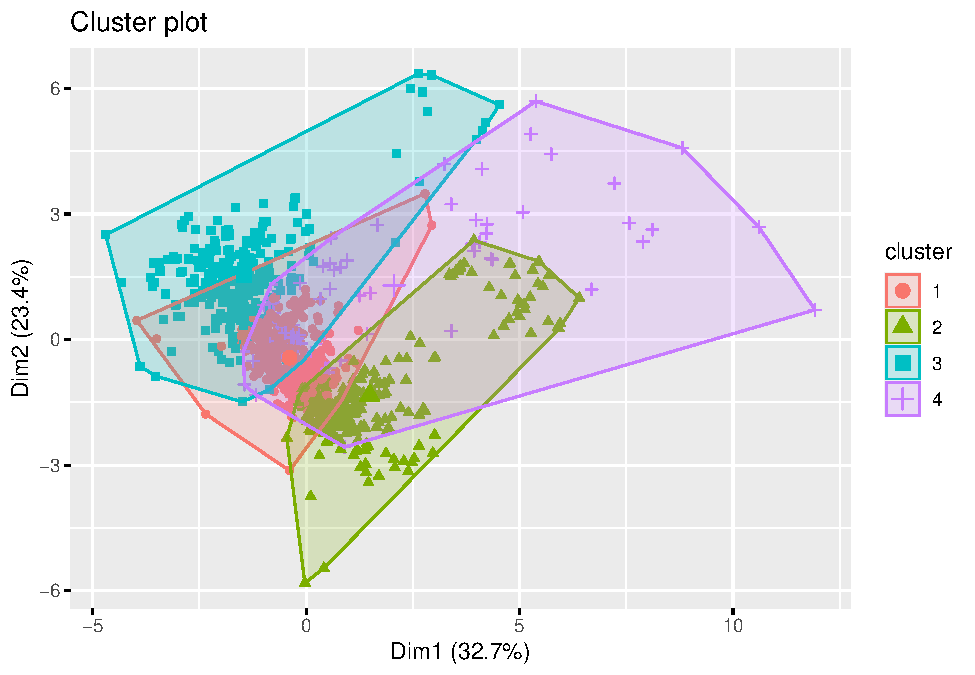
\includegraphics{TP2_files/figure-latex/unnamed-chunk-28-1.pdf} On
remarque qu'une des classes (noire) est isolée par rapport aux deux
autres qui sont regroupées (verte et rouge).

\end{document}
